\section{Programming: Missing Data Imputation}
For this question, refer to the Jupyter Notebook. You will be implementing different imputation techniques -- the notebook will have detailed instructions.

\subsection{Zero Imputation}
Look for the code marked \verb|#TODO| in the notebook and complete the code between the segments according to the instructions. \\

\begin{itemize}
    \item 
Add the accuracy and the Frobenius norm in this report.

\begin{table}[H]
\centering
\begin{tabular}{ |c|c| } 
 \hline
 Frobenius Norm & 51.668 \\
 Accuracy & 60.0\% \\
 \hline
\end{tabular}
\caption{Accuracy and Frobenius norm for Zero Imputation}
\label{nnOA}
\end{table}

\item
Add the code of the completed zeroImpute method. 
\begin{lstlisting}[language = Python, caption=zeroImpute method]
def zeroImpute(X_miss):
  '''
  Returns :
  X_imputed which has zeroes instead of missing values and same shape as X_miss.
  '''
  X_imputed = X_miss.copy()

  # replace missing values with zeroes
  X_imputed = np.nan_to_num(X_imputed)

  assert X_imputed.shape == X_miss.shape

  return X_imputed
\end{lstlisting}


\end{itemize}


\subsection{Mean Imputation}
Look for the code marked \verb|#TODO| in the notebook and complete the code between the segments according to the instructions. \\

\begin{itemize}
    \item 
Add the accuracy and the Frobenius norm in this report.

\begin{table}[H]
\centering
\begin{tabular}{ |c|c|c| } 
 \hline
 Frobenius Norm & 13.7633 \\
 Accuracy & 84.0\% \\
 \hline
\end{tabular}
\caption{Accuracy and Frobenius norm for Mean Imputation}
\label{nnOA}
\end{table}


\item
Add the code of the completed meanImpute method. 
\begin{lstlisting}[language = Python, caption=meanImpute method]
def meanImpute(X_miss):
  '''
  Returns :
  X_imputed which has mean of the corresponding column instead of the missing values and same shape as X_miss.
  '''
  X_imputed = X_miss.copy()

  # replace the value of NaNs with the mean of their column.
  X_imputed = np.apply_along_axis(lambda val: 
                                  np.nan_to_num(val, nan=np.nanmean(val)),
                                  0, X_imputed) 

  assert X_imputed.shape == X_miss.shape

  return X_imputed
\end{lstlisting}

\end{itemize}

\subsection{Regression Imputation}
Look for the code marked \verb|#TODO| in the notebook and complete the code between the segments according to the instructions. \\

\begin{itemize}
    \item 
Complete the following table.



\begin{table}[H]
\centering
\begin{tabular}{ |c|c|c| } 
 \hline
 \textbf{Epoch} & \textbf{Frobenius Norm} & \textbf{Accuracy} \\
 \hline
 After Base Imputation & 51.668 & 60.0\% \\
 1 & 23.930 & 74.0\% \\
 2 & 13.986 & 84.0\% \\
 3 & 11.394 & 86.0\% \\
 4 & 10.490 & 90.0\% \\
 5 & 10.047 & 92.0\% \\
 \hline
\end{tabular}
\caption{Accuracy and Frobenius norm for Zero Imputation}
\label{nnOA}
\end{table}


\item Plot for Accuracy for Regression based imputation vs. Number of Features imputed\\
    \begin{figure}[H]
    	\centering
    	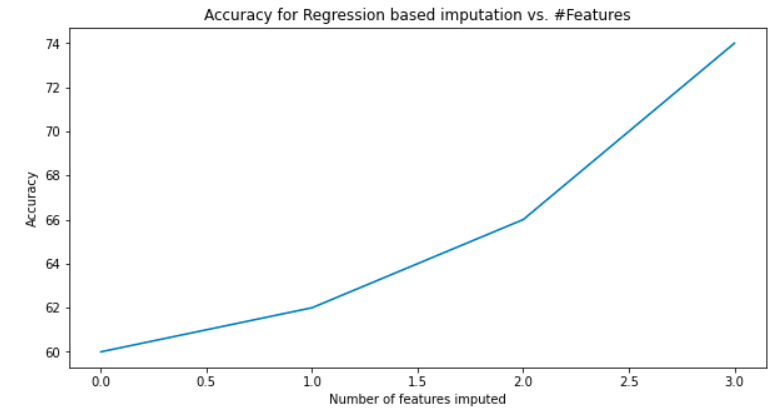
\includegraphics[width=.7\textwidth]{templates/accuracy_vs_features}
    	\label{fig:my_label}
    \end{figure}

\item Plot for Norm for Regression based imputation vs. Number of Features imputed\\
    \begin{figure}[H]
    	\centering
    	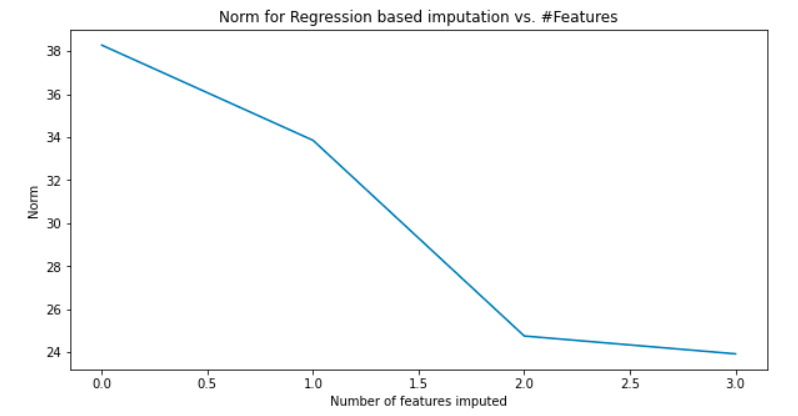
\includegraphics[width=.7\textwidth]{templates/norm_vs_features}
    	\label{fig:my_label}
    \end{figure}

\item Plot for Accuracy for Regression based imputation vs Number of Epochs\\
    \begin{figure}[H]
    	\centering
    	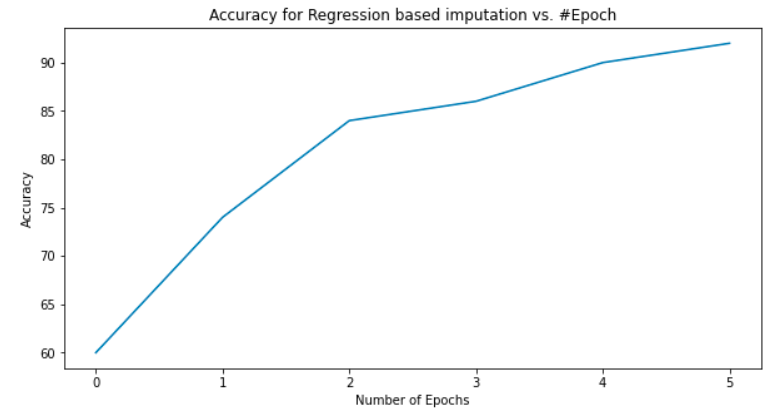
\includegraphics[width=.7\textwidth]{templates/accuracy_vs_epoch}
    	\label{fig:my_label}
    \end{figure}

\item Plot for Norm for Regression based imputation vs. Number of Epochs\\
    \begin{figure}[H]
    	\centering
    	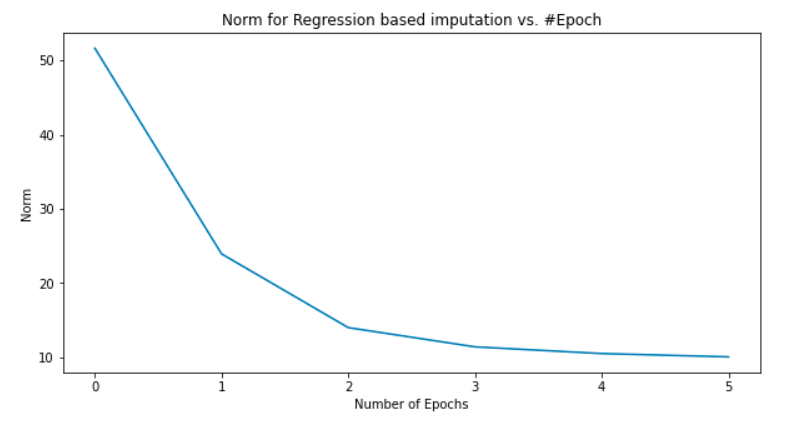
\includegraphics[width=.7\textwidth]{templates/norm_vs_epoch}
    	\label{fig:my_label}
    \end{figure}

\item
Add the code of the completed regressedImpute method. 
\begin{lstlisting}[language = Python, caption=regressedImpute method]
def regressedImpute(X_baseImputed, X_miss, 
                    X_test, y_test, computePerFeatureStatistics = False):
    '''
    Returns :
    X_imputed which has mean of the linearly regressed value instead of the 
    missing values and same shape as X_miss.

    if computePerFeatureStatistics is True, also:
    list of Frobenius norms of difference between reconstructions and original data 
    (without missing values) calculated after each imputing each column.
    list of accuracies on test set of Logistic Regression classifier trained 
    on imputed data after each imputing each column.
    '''
    X_imputed = X_baseImputed.copy()
    frobenius_norms =[]
    accuracies =[]
    
    # We do a linear regression based imputation here, for each column, train a 
    # classifier to predict its value based on values of other features and
    # replace the NaN with the predicted values. 
    # IMPORTANT : You should not use regressed values from an earlier column to predict 
    #             a later column, make sure to train the regression model on base 
    #             imputed and not modify base imputed during the run.
    #             You can use X_miss to find which values were originally NaNs.
    
    for i in range(X_baseImputed.shape[1]):
        
        nan_ix = np.isnan(X_miss[:, i])
        x_train = np.delete(X_baseImputed, i, axis=1)
        y_train = X_baseImputed[:, i]
        
        m = LinearRegression()
        m.fit(x_train, y_train)
        pred = m.predict(x_train)
        
        X_imputed[nan_ix, i] = pred[nan_ix]

        if computePerFeatureStatistics == True:
            clf = LogisticRegression()
            clf.fit(X_imputed, y_miss)
            accuracies.append(clf.score(X_test, y_test))
            frobenius_norms.append(LA.norm(X_train - X_imputed))
            

    if computePerFeatureStatistics == True:
        return X_imputed, frobenius_norms, accuracies
    else:
        return X_imputed
\end{lstlisting}
\end{itemize}


\subsection{Follow Up Questions}
\begin{enumerate}

    
    \item  Which is the best of the three imputation methods? Why (briefly)?
    	\newline \newline
    	The Linear Regression imputation technique is the best of the three considered above since it yields the highest accuracy and smallest Frobenius norm in the test set.
     
      \item Could you potentially do a better job of imputation if you also used y vales as well as x's? How might that help? If using the y's for imputation helps, why do people mostly not use them?
      \newline
      \newline
      To answer the last question, $Y$ is generally  not used to predict $X$ because this can very quickly lead to over-fitting, since when we try to generalize this model and run it on the test set, we will not have access to the test labels by design. 
      \newline
      \newline
      Generally, $Y$ is correlated with $X$, so using the labels to impute missing inputs can lead to better performance. However, due to the above considerations, this is not a good strategy.
         
    \item Describe the trend for the accuracy and the norm as impute more features for regression imputation. Give a plausible explanation behind the trend.
    \newline
    \newline
	The general trend as we impute more features for regression is that the Frobenius norm decreases and the accuracy of our imputations increases.
    \newline
    \newline
    As we impute more features, we learn more about the original distribution used to create $X$. This added information about the latent distribution makes our norm shrink and the predictive power of $Y$ increase.    
    \item Describe the trend for the accuracy and the norm as re-impute again for several epochs for regression imputation. Give a plausible explanation behind the trend.
        \newline
        \newline
    	The general trend as we re-impute features for several epochs in the regression is that the Frobenius norm decreases and the accuracy of our imputations increases.
        \newline
        \newline
	This is caused by the fact that with each epoch, the regressor uses the past approximation of $X$ to generate the next one, causing the approximation to improve with each epoch.    
    
\end{enumerate}